% !TeX root = ./paper.tex
\documentclass[modern]{aastex62}

% Load the corTeX style definitions
% !TeX root = ./ms.tex
% All the packages
\usepackage{url}
\usepackage{amsmath}
\usepackage{mathtools}
\usepackage{amssymb}
\usepackage{natbib}
\usepackage{graphicx}
\usepackage{calc}
\usepackage{etoolbox}
\usepackage{xspace}
\usepackage[T1]{fontenc} % https://tex.stackexchange.com/a/166791
\usepackage{textcomp}
\usepackage{ifxetex}
\ifxetex
\usepackage{fontspec}
\defaultfontfeatures{Extension = .otf}
\fi
\usepackage{fontawesome}
\usepackage{listings}
\usepackage{nicefrac}
\usepackage[bb=boondox]{mathalfa}
\usepackage{booktabs}
\usepackage{longtable}

% Shorthand for this paper
\newcommand{\starry}{\textsf{starry}\xspace}
\newcommand{\Python}{\textsf{Python}\xspace}
\newcommand{\cpp}{\textsf{C}++\xspace}
\newcommand{\bvec}[1]{{\ensuremath{\mathbf{#1}}}}
\newcommand{\xxx}[1]{{\color{red}#1}}
\DeclarePairedDelimiter\floor{\lfloor}{\rfloor}
\DeclarePairedDelimiter\ceil{\lceil}{\rceil}
\newcommand{\imag}{{\ensuremath{\mathbb{i}}}}
\newcommand{\quadquad}{\quad\quad\quad\quad}

\newcommand{\R}{\bvec{R}}
\newcommand{\AOne}{\bvec{A_1}}
\newcommand{\alm}{\bvec{a}}
\newcommand{\x}{\bvec{x}}
\newcommand{\D}{D}
\newcommand{\Doppler}{\bvec{D}}
\newcommand{\Surf}{\mathcal{S}}
\newcommand{\Curve}{\mathcal{C}}
\newcommand{\Dargs}{\bvec{d}}
\newcommand{\lmax}{\ensuremath{l_\mathrm{max}}}
\newcommand{\spot}{\texttt{SPOT}\xspace}
\newcommand{\vogtstar}{\texttt{VOGTSTAR}\xspace}
\newcommand{\kT}{\boldsymbol{\kappa}^\top}
\newcommand{\rhoT}{\boldsymbol{\rho}^\top}
\newcommand{\ylmbasis}{\boldsymbol{\psi}^\top}
\newcommand{\pbasis}{\boldsymbol{\phi}^\top}
\newcommand{\pbasisn}{\ensuremath{\phi_n}}
\newcommand{\azero}{\ensuremath{\bvec{a_0}}}

% References to text content
\newcommand{\documentname}{\textsl{article}}
\newcommand{\figureref}[1]{\ref{fig:#1}}
\newcommand{\Figure}[1]{Figure~\figureref{#1}}
\newcommand{\figurelabel}[1]{\label{fig:#1}}
\renewcommand{\eqref}[1]{\ref{eq:#1}}
\newcommand{\Eq}[1]{Equation~(\eqref{#1})}
\newcommand{\eq}[1]{\Eq{#1}}
\newcommand{\eqalt}[1]{Equation~\eqref{#1}}

% Add code, proof, and animation hyperlinks
\definecolor{linkcolor}{rgb}{0.1216,0.4667,0.7059}
\newcommand{\codeicon}{{\color{linkcolor}\faFileCodeO}}
\newcommand{\prooficon}{{\color{linkcolor}\faPencilSquareO}}
\newcommand{\codelink}[1]{\href{https://github.com/user/repo/blob/cfda45841cf4235e82cf705ab27251bd783bdf8c/tex/figures/#1.py}{\codeicon}\,\,}
\newcommand{\animlink}[1]{\href{https://github.com/user/repo/blob/cfda45841cf4235e82cf705ab27251bd783bdf8c/tex/figures/#1.gif}{\animicon}\,\,}
\newcommand{\prooflink}[1]{\href{https://github.com/user/repo/blob/cfda45841cf4235e82cf705ab27251bd783bdf8c/tex/proofs/#1.ipynb}{\raisebox{-0.1em}{\prooficon}}}
\newcommand{\cilink}[1]{\href{https://dev.azure.com/user/repo/_build}{#1}}


% Define a proof environment for open source equation proofs
\newtagform{eqtag}[]{(}{)}
\newcommand{\currentlabel}{None}
\newenvironment{proof}[1]{%
\ifstrempty{#1}{%
\renewtagform{eqtag}[]{\raisebox{-0.1em}{{\color{red}\faPencilSquareO}}\,(}{)}%
}{%
\renewtagform{eqtag}[]{\prooflink{#1}\,(}{)}%
}%
\usetagform{eqtag}%
\renewcommand{\currentlabel}{#1}
\align%
}{%
\endalign%
\renewtagform{eqtag}[]{(}{)}%
\usetagform{eqtag}%
\message{<<<\currentlabel: \theequation>>>}%
}

% Display the runtime on Azure
\usepackage[skins]{tcolorbox}
\newtcbox{\figtimebox}{enhanced,nobeforeafter,tcbox raise=-0.8mm,boxrule=0.6pt,
  top=0.5mm,bottom=0mm,right=0mm,left=6mm,arc=1pt,boxsep=2pt,
  before upper={\vphantom{dlg}},colframe=linkcolor,coltext=linkcolor,
  fontupper=\sffamily\bfseries\tiny,colback=white,overlay={\begin{tcbclipinterior}
  \fill[linkcolor] (frame.south west)
  rectangle node[text=white,font=\sffamily\bfseries\tiny,rotate=0]{CPU} 
  ([xshift=6mm]frame.north west);\end{tcbclipinterior}}}
\robustify{\figtimebox}
\pdfstringdefDisableCommands{%
  \def\figtimebox#1{'#1'}%
}
\newcommand{\figtime}[1]{\IfFileExists{figures/#1.py.time}%
{%
\cilink{\figtimebox{\input{figures/#1.py.time}\unskip s}}
}{}}

% Define the `oscaption` command for open source figure captions
\newcommand{\oscaption}[2]{\caption{#2 \codelink{#1} \figtime{#1}}}

% Code examples
\definecolor{codegreen}{rgb}{0,0.6,0}
\definecolor{codegray}{rgb}{0.5,0.5,0.5}
\definecolor{codepurple}{rgb}{0.58,0,0.82}
\definecolor{backcolour}{rgb}{0.95,0.95,0.95}
\lstdefinestyle{mystyle}{
    backgroundcolor=\color{backcolour},
    commentstyle=\color{codegreen},
    keywordstyle=\color{magenta},
    numberstyle=\tiny\color{codegray},
    stringstyle=\color{codepurple},
    basicstyle=\small\ttfamily,
    breakatwhitespace=false,
    breaklines=true,
    captionpos=b,
    keepspaces=true,
    numbers=left,
    numbersep=5pt,
    showspaces=false,
    showstringspaces=false,
    showtabs=false,
    tabsize=2,
    aboveskip=1em,
    belowskip=1em,
    keywords=[2]{map},
    keywordstyle=[2]{\color{black!80!black}},
    upquote=true
}
\lstset{style=mystyle}

% Typography obsessions
\setlength{\parindent}{3.0ex}
\renewcommand\quad{\hskip\fontdimen3\font}

% https://tex.stackexchange.com/a/184474
\usepackage{stackengine,scalerel}
\def\lnlam{\ThisStyle{\ensurestackMath{\stackon[-2.4\LMpt]{%
  \SavedStyle\lambda}{\kern-.5pt\kern\LMpt\rule{1\LMex}{.25pt+.15\LMpt}}}}}

% Bibliography stuff
\bibliographystyle{aasjournal}
\setlength\LTcapwidth{\textwidth}
\begin{document}

% Title
\title{Occultation mapping of Io's surface in the near-infrared I: Inferring static maps} 

% Author list
\author{Fran Bartoli\'c}
\email{fbartolic@flatironinstitute.org}
\affil{Center~for~Computational~Astrophysics, Flatiron~Institute, New~York, NY}
\affil{Centre for Exoplanet Science, SUPA, School of Physics and Astronomy, University of St. Andrews, St. Andrews, UK}
\author{Rodrigo Luger}
\author{Daniel Foreman-Mackey}
\affil{Center~for~Computational~Astrophysics, Flatiron~Institute, New~York, NY}
%

\begin{abstract}
Jupiter's moon Io is the most volcanically active body in the Solar System with hundreds of active volcanoes varying in intensity on different timescales.
Existing photometric observations in the near infrared taken during occultations by Jupiter and other Galilean moons encode a wealth of information about its surface.
These data are ideal for testing methods for inferring surface features of occulted bodies from time series observations.
We built a generative model of Io's surface using the code starry \href{https://rodluger.github.io/starry/}{\color{linkcolor}\faGithub} which enables fast analytic and differentiable computation of occultation light curves in emitted and reflected light.
    Our fully Bayesian model is able to recover known bright features on the surface of Io with only two light curves and without any assumptions on where the features are located or how many there are.
    The methods we have developed are also directly applicable to the problem of mapping stars and exoplanets.\href{https://github.com/fbartolic/volcano}{\color{linkcolor}\faGithub}
\end{abstract}

%
\section{Introduction}
The surface of Jupiter's moon Io is littered with hundreds of volcanoes which appear as bright spots in the near infrared and in intensity on timescales ranging from days to decades.
The volcanic activity is driven by tidal interactions with Jupiter and sustained by the Laplace resonance with Europa and Ganymede \citep{peale1979}.
Because of its extreme volcanic activity, Io is in many ways an analogue of a volcanically active exoplanet.
Volcanic exoplanets, often dubbed \emph{super-Ios} or \emph{lava worlds}, have gathered a lot of interest in recent years because both photometric and spectral signatures of volcanic activity on such worlds will likely be detectable in the near future with telescopes such as JWST and LUVOIR \citep{kaltenegger2010,henning2018,oza2019}.
Studying extreme volcanism on both Io and exoplanets is scientifically valuable because it provides a window into the properties of the early Earth and it informs theories of planet formation.

Existing exoplanet detections with potential volcanism include CoRoT-7b \citep{barnes2010}, the first rock exoplanet to have been discovered and one which likely heated by strong tidal forces; 55 Cancri e, whose inferred longitudinal offset in peak surface emission has been attributed to, among other things, lava flows on the surface \citep{demory2016,demory2016a,hammond2017}; several planets in the TRAPPIST-1 system in a Laplace-like resonance with likely volcanic activity \citep{kislyakova2017,dobos2019} and many others.
Not all exoplanets will have Io-like volcanism, some will have magma oceans due to their proximity to the star or volcanism caused by nuclear decay similar to early Earth volcanism.

Io has been observed extensively using both space and ground observatories.
High resolution images of Io's surface were taken by space missions such as Voyager \citep{smith1979}, Galileo \citep{belton1996} and Juno \citep{mura2020}.
It has also been resolved from the ground in the near infrared using disk resolved imaging
\citep{howell1985,simonelli1986,spencer1990} and adaptive optics observations \citep{marchis2000,marchis2005,dekleer2016}.
Most importantly for this work, Io has been sporadically observed for decades using high cadence near infrared photometry taken during occultations by Jupiter starting with \cite{spencer1990}.
Occultations by Jupiter occur twice every orbit lasting ~1.7 days and mutual occultations with Europa, Ganymede or Callisto happen every ~6 years when Earth pasess through the orbital plane of Galilean satellites.
The majority of occultations by Jupiter are observed when Io is in Jupiter's shadow ("in eclipse") while mutual occultations are almost always observed in sunlight because mutual occultations while Io is in eclipse are extraordinarily rare.
Only the brightest volcanoes are visible over the reflected light background when Io is illuminated by the Sun\citep{veeder1994,dekleer2016a}.

Both kinds of occultations have been used to study volcanic activity on the surface.
\cite{spencer1994} observed several occultations of Io by Europa and detected a major brightening of the most powerful of Io's volcanoes, Loki, relative to previous Voyager observations.
\cite{rathbun2002, rathbun2006,rathbun2010} used observations from NASA's IRTF telescope to study the long term variability of different volcanic spots finding evidence of periodicity in Loki's eruptions and established the transient nature of the volcanoes (only Loki is persistently active).
By studying an occultation of Io by Europa, \cite{dekleer2017} mapped the Loki region to a precision of about 2 kilometers.
In addition to observations of occultations in near infrared, several groups have been observing mutual occultations in the optical \citep[][and references therein]{arlot1974,saquet2018,morgado2016a} for decades with the purpose of inferring the optical albedo of Io and improving ephemeris precision for Galilean satellites.

None of the studies of occultations in the infrared attempted to infer a two-dimensional map of Io's surface.
The light curves are usually fit independently with the goal of inferring one-dimensional longitudinal variations in brightness on its surface.
Strong priors on the locations of individual volcanoes are assumed based on maps from space mission observations.
In this work, we build a fully probabilistic model in order to infer a two-dimensional \emph{map} of Io's volcanic surface from archival IRTF observations in the near infra red.
We assume that the map generating a given set of light curves is static (up to an overall amplitude) so we are restricted to modeling the surface during a timespan when the surface emission hasn't changed drastically.
In a subsequent paper we build on the model we have developed here and generalize to a case where the surface is time-variable.

The model is built on top of the recently developed code starry \citep[][Luger et al. 2020 in prep]{luger2019a} which enables fast analytic computation of occultation light curves and phase curves for objects whose surface features are represented in terms of spherical harmonics.
Starry can compute phase curves and occultations in both emitted light (for modeling the isotropic thermal emission from Io's surface) and reflected light (for mapping albedo variations).
It is many orders of magnitude faster and more accurate than pixel based codes and it computes exact gradients with respect to all parameters through automatic differentiation.
Starry also comes with extensive tools for visualizing spherical harmonic maps and simulating data.

Our goal for this paper is to develop a general model for mapping surfaces of occulted bodies with sparse high contrast features and to test it on a real world dataset. 
Because we have lots of prior information on what the surface of Io should look like, we can compare our inferences to known features on its surface and we can test the sensitivity of the inferred maps to different choices of priors and noise models.
The work should also be of interest to the Io research community as it presents a very different approach to modeling Io occultations without having to make strong assumptions on the locations of the hot spots. 

The paper is organized as follows.
In \S\ref{sec:data} we describe the IRTF light curves of occultations by Jupiter which we use to infer maps.
In \S\ref{sec:model} we discuss the generative model for the data and we write down the relevant likelihood functions.
In \S\ref{sec:inverse_problem} we focus on the question of how to do Bayesian inference given the forward model specifications defined in \S\ref{sec:model}.
We discuss and test different priors on map features, the information content of light curves and fitting the modelsusing Hamiltonian Monte Carlo (HMC). 
We show results on simulated data.
\S\ref{sec:results} shows the results on real IRTF data for two pairs of light curves (closely spaced in time)
In particular, the inferred dynamic map, the  different component maps and accompanying coefficients, the uncertainties of the maps, sensitivity to different choices of priors, comparison of inferred locations and intensities of spots to known values from the literature.
Finally, in \S\ref{sec:exoplanets} we discuss applications of the model to future exoplanet obervations and test the model predictions on simulated JWST observations of a volcanic Super-Earth.

\section{Data}
\label{sec:data}

\begin{figure}[h!]
    \begin{centering}
    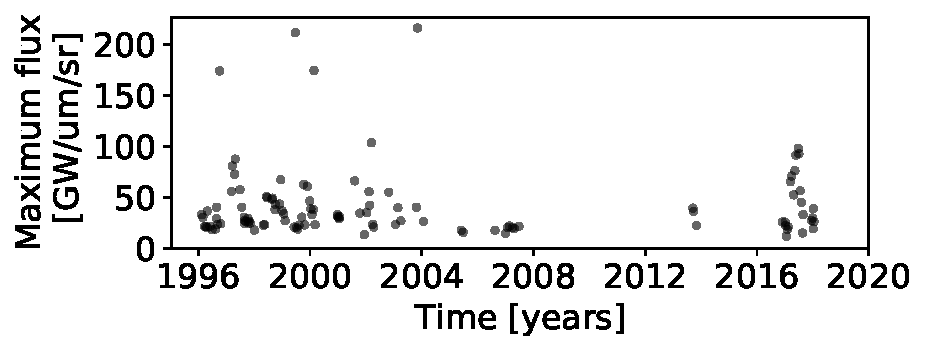
\includegraphics[width=\linewidth]{figures/irtf_max_flux.pdf}
    \oscaption{irtf_dataset}{%
        Maximum flux for each IRTF light curve of Io observed during an occultation of Io by Jupiter.
       \label{fig:irtf_max_flux}
    }
    \end{centering}
\end{figure}

The dataset we use to infer maps of Io's surface consists of 112 observations of Io in the near infrared taken from 1996 until 2018 using different instruments at NASA's IRTF observatory, the NSFCam  1-5 $\mu m$ camera \citep{shure1994} (TODO: WHICH FILTERS), the SpeX 0.8-5.5 $\mu m$ spectrographer/imager \citep{rayner2003} (TODO: DETAILS) and the iShell 1.1-5.3 $\mu m$  spectrographer/imager \citep{johnrayner2016}.
Although the observations span decades, the cadence is non-uniform, there are only a few observations taken between 2008 and 2016.
All of the observations were taken while Io was \emph{in eclipse}, meaning that it was in Jupiter's shadow and all of the observed emission from the surface is due to thermal radiation.
Observations of Io \emph{in sunlight} on the other hand probe both the thermal (volcanic) emission and the surface albedo variations in the near infrared.
Figure~\ref{fig:irtf_max_flux} shows the maximum flux in units of $\mathrm{GW}/\mu \mathrm{m}/\mathrm{sr}$ (TODO: UNDERSTAND THESE UNITS) for each light curve plotted as a function of time.
This value is approximately equal to the total flux emitted from the Jupiter facing side of Io.
The baseline brightness is varying stochastically by a large amount and there are several notable events of intense volcanic activity.

\begin{figure}[h!]
    \begin{centering}
        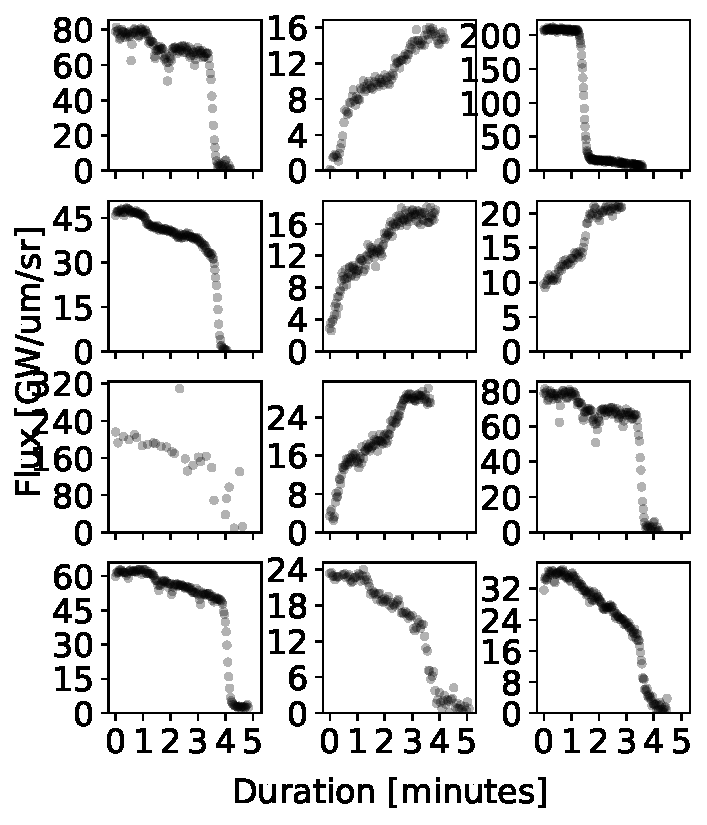
\includegraphics[width=0.7\linewidth]{figures/irtf_sample_lightcurves.pdf}
    \oscaption{irtf_dataset}{%
        A selection of sample light curves taken during occultations of Io by Jupiter in our dataset.
        The step-like morphology of the light curves is due to bright volcanoes on Io's surface coming in or out of view during an occultation.
        These light curves thus visibly encode information about the features on the surface.
        \label{fig:irtf_sample_lightcurves}
    }
    \end{centering}
\end{figure}

In Figure~\ref{fig:irtf_sample_lightcurves} we display a random subset of all the light curves
in the dataset.
All occultations last for $\sim4$ min.
The exposure cadence for each light curve is around a second with some variation between light curves.
It follows that over the course of a single exposure Jupiter's limb passes over about 15km on Io's surface which provides a lower bound for the size of the features that we can reliably estimate.
The shapes of light curves strongly deviate from the smooth variability one would expect assuming uniform thermal surface emission.
Especially prominent are light curves with clear step-like features which are present when bright localized spots come in or out of view during the course of an occultation.
The fact that these features are so clearly visible means that even individual light curves encode precise information on the longitudinal position of the spots.

The photometric quality of the light curves varies from year to year because multiple instruments were used over the years. 
As with all ground based photometry, the observations are influenced by atmospheric variability which results in some correlated noise in the light curves and because of this the flux is not always monotonically increasing or decreasing as one would expect.
The light curves lack errorbars. 
To estimate the errorbars we do some basic pre-processing on the light curves. 
We filter each light curve with the Savitzky-Golay filter as implemented in \textsf{SciPy} \citep{virtanen2020} with
a third order polynomial and a window length equal to 5\% of the number of data points and rounded up to the nearest odd integer. 
After filtering, we compute the residuals with respect to the filtered model and run iterative sigma-clipping, removing all data points 5 median absolute deviations (MAD) from the median value. 
Finally, we estimate the errorbars by computing the standard deviation of the sigma clipped residuals.
This estimate is far from perfect which is why we introducing a rescaling parameter when fitting the model.


\section{Model}
\label{sec:model}
\subsection{Orbital parameters}
\label{ssec:orbital_parameters}
To model the occultations we need to know the projected relative position of Jupiter with respect to Io and the orientation of Io at any given time.
To compute the geometry, we use the \href{https://ssd.jpl.nasa.gov/horizons.cgi}{JPL Horizons database} and the latest planetary ephemeris DE430 \citep{folkner2014} which is accurate to a few kilometers on Io's surface.
For both Jupiter and Io we need the Right Ascension and Declination and the angular (equatorial) diameter (\textsf{Ang-diam}).
In addition, we need to fix the orientation of Io we need the longitude and the latitude at the center of Io's disc as seen from Earth (\textsf{Ob-lon}, \textsf{Ob-lat}) and the counterclockwise angle between the Celestial North Pole unit vector projected onto the plane of the sky and the Io's north pole (\textsf{NP.ang}).
All longitudes are positive  in the direction of West.
\textsf{HORIZONS} provides all ephemeris with a minimum cadence of 1 second so we interpolate all values so that we can evaluate them for arbitrary times.

The coordinate system in \textsf{starry} is defined to be right handed such that the $\hat{z}$
axis points towards the observer and the $\hat{x}$ axis points to the right on the plane of the sky.
The radius of the occulted sphere is fixed to 1 and the orientation is specified by three angles,
the counterclockwise obliquity angle \textsf{obl} between the $\hat{y}$ axis and the North Pole of the sphere, the inclination angle \textsf{inc} which is set to $90^\circ$ if the North Pole is aligned with the $\hat{y}$ axis and the phase angle \textsf{theta} which rotates the sphere around the $\hat{y}$ axis in the eastward direction.
We have $\mathrm{obl}=\textsf{NP.ang}$, $\mathrm{inc}=90^\circ-\textsf{Ob-lat}$ and
$\mathrm{theta}=\textsf{Ob-lon}$.
The occultor position relative to the occulted object is given by
\begin{align}
    \mathrm{xo}/\gamma&=-\Delta\alpha\,\cos\delta\\
    \mathrm{yo}/\gamma&=\Delta\delta\\
    \mathrm{zo}/\gamma&=1
\end{align}
where $\Delta\alpha$ and $\Delta\delta$ are differences in Right Ascension and Declination respectively relative to the occulted object and $\gamma$ is the angular radius of the occulted sphere.

\subsection{Jupiter's effective radius}
Although the sky position of Jupiter relative to Io is known to a precision of a few kilometers, several complications arise when attempting to compute Jupiter's radius.
First, Jupiter is not spherical and its equatorial radius is greater than the polar radius by thousands of kilometers. 
Because \textsf{starry} does not support occultations by non-spherical occultors and because the effect is negligible at the resolution of our maps, we assume that Jupiter is locally spherical at the point of an occultation. 
We estimate an effective radius from the measurements of Jupiter's shape from Voyager radio occultation data \citep{lindal1981}.
These data come in the form of a plot of effective radius  as a function of Jupiter's planetocentric latitude at a fixed pressure of 100 mbar \citep[Fig.~7 in ][]{lindal1981}.
When computing the occultation latitude we fix Jupiter's latitude to the value at the center of Io's disc because 
the variation of Jupiter's effective radius along Io's disc is negligible.


Second, Jupiter is gaseous so it does not have a well defined boundary.
In principle, we should compute an effective radius of Jupiter at different locations (pressure) in the atmosphere and model an occultation of Io by a fuzzy occultor.
Although this is possible with Starry, it is unnecessary for our models because the characteristic scale height of Jupiter is around 27 km (CITE) which is below the uncertainty of our inferred maps.
Instead, we follow the approach in \cite{spencer1990} and compute the effective radius of Jupiter at about 2.2 mbar, the pressure (and the associated effective radius) at which a  bright source on the surface of Io fades by 50\% due to differential refraction during the course of an occultation.

Third, the information on the effective radius in \citep{lindal1981} is provided only at a fixed pressure of 100 mbar.
To adjust the values for a lower pressure of 2.2 mbar we assume an exponential pressure profile $P=P_0\, e^{-\Delta r/H}$ where $H$ is the scale height and $\Delta r$ is the height difference between the two pressure levels.
It follows that to convert the shape profile at 100 mbar to 2.2 mbar we need to add the factor
$-H\ln(2.2/100)$ which is assumed to be constant in the $\pm 21$ deg latitude range in which the occultations occur.
In addition to refractive absorption in Jupiter's atmosphere there is a also slight additional molecular absorption due to methane which \cite{spencer1990} estimate to be equal to around 12\% in their filter, we choose to ignore this because it is far below the resolution of our maps.

Finally, we have to account for the fact that the light from Io is getting significantly bent at the point of half reflective intensity in Jupiter's atmosphere which results in a smaller shadow of Jupiter on the surface of Io then would be the case for a straight propagation.
It is zero at the beginning of the disappearance of a hot spot when there is no refraction, increasing to one scale height $H$ at the half intensity point and then increasing further to a large value when Io disappears behind Jupiter's limb.
We ignore the variation in the bending and adopt a fixed value of one scale height for this effect which we subtract from the value of the effective radius.

In summary, to compute an effective radius of Jupiter for a given occultation of Io first we have to compute Jupiter's planetocentric latitude at which Io's disk disappears or reappears behind the limb, then use a modified shape profile from \cite{lindal1981} to get an effective radius and finally we have to subtract one scale height due to light bending.
There are substantial uncertainties in each of these steps.
The data about on the shape profile are quite old and it is not known if the structure of Jupiter's atmosphere stayed the same since 1980s. 
The shape profile also depends on the wind velocity structure and temperature which we do not take into account.
In addition to uncertainties about the atmospheric structure, there are uncertainties associated with digitizing the data shown in Fig.~7 in \cite{lindal1981} because it is not available in table form.
We digitized the figure by reading off the data points "by eye" and then interpolating them using cubic spline interpolation.

Throughout this paper the highest resolution maps we fit to the data are of order $l=25$ which corresponds to a characteristic length scale of around 230 km on the surface of Io.
This is about an order of magnitude larger than the errors introduced in the effective radius estimate above so we are not concerned with substantial errors in our radius estimate.

\subsection{Model specification}
\label{ssec:model_spec}
Given the geometry of on occultation event at an arbitrary time, computing the predicted flux with \textsf{starry} is straightforward.
\textsf{starry} computes the integrated flux of an unocculted or an occulted sphere analytically assuming that the surface map can be expanded in terms of spherical harmonics $Y_{lm}(\theta,\phi)$ up to a certain \emph{degree} $l$.
The map is thus defined by a vector of spherical harmonic coefficients $\mathbf{y}$ which multiplies the spherical harmonic basis $\tilde{\mathbf{y}}(x, y)=\left(Y_{0,0} Y_{1,-1} Y_{1,0} Y_{1,1} Y_{2,-2} Y_{2,-1} Y_{2,0} Y_{2,1} Y_{2,2} \cdots\right)^{\top}$ and the total number of coefficients is $(l+1)^2$.
In addition to computing \emph{thermal} phase curves and occultation light curves, \textsf{starry} also solves the considerably more complex problem of computing reflected light phase curves and occultations when the sphere is illuminated by a distant light source \citep[Luger et al. 2020 in prep][]{} which is complicated by the presence of the terminator line.
In the case of a reflected light map, the coefficient vector $\mathbf{y}$ represents spherical albedo in a given wavelength range.
We only use data taken while Io was in eclipse shadowed by Jupiter so we do not need to model the reflected light component. 
If instead we had occultation data or phase curves taken while Io is illuminated by the Sun and if both the thermal component and the reflected sunlight component of observed flux were comparable, it would be necessary to simultaneously fit for two vectors of spherical harmonic coefficients, 
one for the albedo distribution and the other for thermal emission.

Importantly, conditional on the parameters specifying the geometry of the occultations being fixed, the \textsf{starry} model is \emph{linear} for both emitted and reflected light maps.
\cite{luger2019} achieved this by representing all rotations, changes of basis transformations and integrals with complicated boundaries which are needed to compute the flux as linear transformations.
Since a sequence of linear mappings is also linear, the predicted flux can be written as
\begin{equation}
    \mathbf{f}=\mathbf{A}\,\mathbf{y}
    \quad,
    \label{eq:linear_model}
\end{equation}
where the column vector $\mathbf{f}$ of shape $(T, 1)$ is the predicted flux for different values of the occultor position and optionally the direction of the illumination source and $\mathbf{A}$ is the design
matrix of shape $(T, N)$ (with $N=(l+1)^2$) which encodes information all operations needed to compute the integrated flux.
If the geometry isn't known precisely then the matrix $\mathbf{A}$ is not fixed and the model is no longer linear.

The characteristic angular scale of features that can be represented with a given map is set by the degree of the map and it is approximately equal to $\frac{180^\circ}{l}$.
For reference, state of the art inferences involving phase curves and secondary eclipses of exoplanets are able to constrain features of order $l=1$ (inferring a bright spot offset from the substellar point) but for Io we need to fit much higher order maps because the typical scale of volcanic spots is on the order of tens of kilometers (a few degrees).
\textsf{starry} can handle maps up to $l\approx 20$ before numerical instabilities kick in (TODO: make this statement more precise).

Although \textsf{starry} is built around the idea of expanding surface features in a spherical harmonic basis, this is not the ideal basis for doing inference because it makes it difficult to ensure that the intensity is positive everywhere on the map.
The positivity constraint is important not only because we want to avoid having unphysical regions on inferred maps but also because it imposes a strong constraint on the map which substantially reduces the complexity of the inference problem.
Unfortunately, there is no analytic way to determine weather a given spherical harmonic map $\mathbf{y}$ is positive-valued everywhere on the sphere. 

The are two ways of circumventing this problem that we are aware of.
The first is to evaluate the intensity on a (sufficiently fine) discrete grid of \emph{pixels} $\mathbf{p}$ on the sphere and then either fit for $\mathbf{y}$ while rejecting steps when fitting the model for which any of the pixels $\mathbf{p}$ end up being negative.
The second is to treat the pixels as model parameters but still compute the actual light curve model in the $Y_{lm}$ basis where everything is fast. 
We opt for the latter approach because it is much easier to implement.
The mapping from spherical harmonics $\mathbf{y}$ to pixels $\mathbf{p}$ can be expressed as a linear operator 
$\mathbf{P}$:
\begin{equation}
    \mathbf{p}=\mathbf{P}\,\mathbf{y}
\end{equation}
Each row of $\mathbf{P}$ contains values of each of spherical harmonic coefficients at a given point on the grid. 
To construct the grid we use an equal area Molleweide projection so that we don't end up with more pixels in some areas of the sphere than others.
The grid needs to be fine enough to ensure positivity over most of the sphere.
We find that we need to have more pixels than spherical harmonics by a factor of at least 4.
This increases the computational cost of the inference somewhat because the number of parameters we have to fit increases fourfold.

Because $\mathbf{P}$ is not a square matrix, we cannot compute its inverse to obtain the inverse transform, however we can still compute the Moore-Penrose pseudoinverse $\mathbf{P}^\dagger$ by solving the linear system $\mathbf{P}\,\mathbf{P}^\dagger=\mathbf{I}$ where $\mathbf{I}$ is the identity matrix. 
The solution is given by
\begin{equation}
\mathbf{P}^\dagger=\left(\mathbf{P}^{\top} \mathbf{P}+\lambda \mathbf{I}\right)^{-1} \mathbf{P}^{\top}
    \quad,
\end{equation}
where $\lambda$ is a small regularization parameter and $\mathbf{I}$ is the identity matrix.
We then have 
\begin{equation}
    \mathbf{y}'=\mathbf{P}^\dagger\mathbf{p}'
\end{equation}
Both matrices can easily be pre-computed with \textsf{starry} before doing inference.
We use the symbol $\mathbf{p}'$ to denote pixels which are mapped to spherical harmonic coefficients using $\mathbf{P}^\dagger$ and $\mathbf{p}$ for those generated from $\mathbf{y}$ using $\mathbf{P}$.
In the rest of the paper we call the former kind of pixels \emph{sphixels}.
Setting $\mathbf{A}'\equiv \mathbf{A}\,\mathbf{P}^\dagger$, we see that the flux is also linear in the spixels:
\begin{equation}
    \mathbf{f}=\mathbf{A}'\,\mathbf{p}'
    \label{eq:linear_model_pix}
\end{equation}

\begin{figure}[h!]
    \begin{centering}
    \includegraphics[width=1.\linewidth]{figures/sphixels_to_pixels.pdf}
    \oscaption{sphixels_to_pixels}{%
        Transformation of a pixelated map in which we set our priors (left) to the spherical harmonic basis which we use to compute the model (middle) and then again to pixels.
        The mapping from spherical harmonics to pixels is exact but the reverse is not true so to differentiate between pixels mapped to spherical harmonics and pixels constructed from spherical harmonics we call the former "sphixels".
        Since there are many more sphixels than there are spherical harmonics coefficients a sphixel map 
       drawn from an Exponential prior on the left can only be approximately represented in the $Y_{lm}$ basis and the effective prior on pixels ends up looking more like a skewed Gaussian with a heavy right tail than an Exponential.
  \label{fig:sphixels_to_pixels}
    }
    \end{centering}
\end{figure}


To visualize the effect of the transformation from sphixels to spherical harmonics, in Figure~\ref{fig:sphixels_to_pixels} we plot a single draw of sphixels $\mathbf{p}'$ from an Exponential prior (left) in the Mollweide projection, map them to spherical harmonics (middle), and then generate another pixelated map from the spherical harmonics on a grid of the same size as the initial sphixel grid.
The middle map is visibly smoother than the prior map and looking at the histograms (black) the effective prior looks more like a skewed Gaussian with a heavy right tail than an Exponential distribution.
There is also minimal leakage into negative values of intensity.
The reason for this is that the pixels $\mathbf{P}\,\mathbf{y}'$ generated from $\mathbf{P}^\dagger\mathbf{p}'$ do not completely respect the Exponential prior because some information is lost in going from sphixels to spherical harmonics.
Nevertheless, in Section~\ref{ssec:sphixels_vs_harmonics} we find that setting priors on sphixels is a far better solution than using the spherical harmonic coefficients.

\subsection{The likelihood}
\label{ssec:likelihood}
Assuming we have a single light curve with $N$ data points and a map specified with sphixels $\mathbf{p}'$, the (Gaussian) log likelihood is given by
\begin{equation}
    \ln\mathcal{L}=-\frac{1}{2}\left[\mathbf{f}_\mathrm{obs}-\mathbf{f} \right]^{\top}
    \boldsymbol{\Sigma}_l^{-1}\left[\mathbf{f}_\mathrm{obs}-\mathbf{f} \right]
    \quad,
    \label{eq:likelihood}
\end{equation}
where $\mathbf{f}_\mathrm{obs}$ is the observed light curve, $\boldsymbol{\Sigma}$ is the data covariance matrix and $\mathbf{f}$ is predicted flux given by
\begin{equation}
    \mathbf{f}=\mathbf{A}'\,\mathbf{p}' +b\,\mathbf{1}_N
    \quad,
    \label{eq:flux_model}
\end{equation}
where we have added a fixed flux offset parameter for each light curve in order to account for stray flux which cannot be attributed to Io.
This flux is mostly due to light emitted from Jupiter (TODO: is this right?).

To model the data covariance $\boldsymbol{\Sigma}$ we use use a Gaussian Process and we compute the likelihood using the fast Celerite method \citep{foreman-mackey2017} as implemented in the \textsf{celerite2} package (CITE).
We use the simple (approximate) Matern 3/2 function which is parametrized by two parameters, a standard deviation parameter $\sigma_\mathrm{GP}$ and a characteristic timescale parameter $\rho_\mathrm{GP}$.
The kernel is given by 
\begin{equation}
    k(\tau)=\sigma_\mathrm{GP}^{2}\left[(1+1 / \epsilon) e^{-(1-\epsilon) \sqrt{3} \tau / \rho_\mathrm{GP}}(1-1 / \epsilon) e^{-(1+\epsilon) \sqrt{3} \tau / \rho_\mathrm{GP}}\right]
    \quad,
\end{equation}
where $\tau=|t_n-t_m|$ and $\epsilon$ controls the quality of the approximation.
A single element of the data covariance matrix $\boldsymbol{\Sigma}$ is then 
\begin{equation}
    \boldsymbol{\Sigma}_{nm}=\sigma_n^2\delta_{nm} + k(\tau\sigma_\mathrm{GP},\rho_\mathrm{GP})
    \quad,
    \label{eq:data_covariance_element}
\end{equation}
where $\sigma_n$ is the errorbar for the n-th data point.
In cases where we fit multiple light curves assume independence and the total log likelihood is the product of individual likelihoods defined in Eq.~\ref{eq:likelihood}.

\section{The inverse problem}
\label{sec:inverse_problem}
Having defined the forward model in the previous section, in this section we describe how to solve the inverse problem in a Bayesian setting.

\subsection{The information content of a light curve}
\label{ssec:information_content}
The mapping problem is famously ill posed meaning that specific linear combinations of spherical harmonic coefficients will be in the nullspace of the linear mapping  $\mathbf{A}$ in Eq.~\ref{eq:linear_model}.
This means that even if we had noiseless observations it would still be impossible to recover certain features.
To recover the greatest information about the surface we need to have some mechanism which breaks the various degeneracies.
With phase curves only we can recover longitudinal variations in emission.
Occultations are a lot better because the limb of the occultor sweeps across the surface of the occulted sphere, thereby exposing or blocking light from different points on the surface.
Best case scenario is having phase curve observations plus a series of occultations by a small occultor at different latitudes and different phases.
Observing phase curves and occultations in reflected light improves the model even more because of the nonuniform illumination profile of the incident radiation and the presence of a day/night terminator line \citep[][Luger et al. 2020 in prep]{luger2019a}.
In some cases for reflected light observations (phase curves of an inclined planet for example) there is no nullspace at all at low degrees of the map.

We can reformulate these statements more precisely by computing a measure of information content of the different kinds of observations.
Given that our model is linear, assuming Gaussian priors on the spherical harmonic coefficients with covariance $\boldsymbol{\Lambda}_\mathbf{y}$ and a Gaussian likelihood, the posterior can be computed analytically and its mean is given by
\begin{equation}
    \widehat{\mathbf{y}}=\boldsymbol{\Sigma}_{\hat{\mathbf{y}}}\left(\mathbf{A}^{\top} \boldsymbol{\Sigma}_{\mathbf{f}}^{-1} \mathbf{f}+\boldsymbol{\Lambda}_{\mathbf{y}}^{-1} \boldsymbol{\mu}_{\mathbf{y}}\right)
    \quad,
\end{equation}
where the posterior covariance matrix $\boldsymbol{\Sigma}_{\hat{\mathbf{y}}}$ is 
\begin{equation}
\boldsymbol{\Sigma}_{\hat{\mathbf{y}}}=\left( \mathbf{A}^{\top} \boldsymbol{\Sigma}_{\mathbf{f}}^{-1} \mathbf{A} +\boldsymbol{\Lambda}_{\mathbf{y}}^{-1}\right)^{-1}
\end{equation}
We define the information content as the variance reduction of the posterior relative to the prior which is called \emph{posterior shrinkage}.
The posterior shrinkage $S$ is defined as
\begin{equation}
S \equiv 1-\lim _{\sigma_{0}^{2} \rightarrow \infty} \frac{\sigma^{2}}{\sigma_{0}^{2}}
    \quad,
\end{equation}
where $\sigma^2_0$ is the prior variance and $\sigma^2$ is the posterior variance for a given spherical harmonic coefficient.
It tells us how well we can constrain a particular coefficient in the limit of infinite SNR observations, posterior shrinkage of 1 means that the data provides perfect information and a posterior shrinkage of 0 means that we didn't learn anything.
In order to compute the posterior shrinkage we first compute the design matrices using \textsf{starry} for different kinds of events a over the course of a single year: occultations by Jupiter, occultations by Europa, Ganymede and Callisto and phase curves.
We take the ephemeris data from \textsf{JPL HORIZONS} and assume that it is known exactly and we also assume all observations are of the emitted light component independent of whether Io is in sunlight or in eclipse because we are interested in constraining the volcanic emission rather than the albedo.

\begin{figure}[h!]
    \begin{centering}
    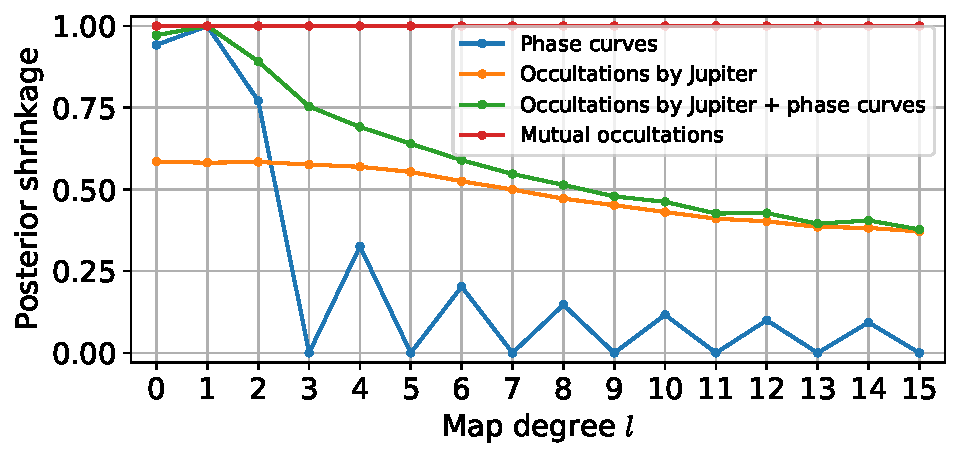
\includegraphics[width=\linewidth]{figures/information_content.pdf}
    \oscaption{InformationContent}{
        The posterior shrinkage for different kinds of observations of Io as a function of spherical harmonic degree (angular scale), averaged across all $m$ modes.
    Posterior shrinkage of 1 represent maximum information gain in updating from the prior to the posterior while 0 represents no information gain. 
    The posterior variance has been computed for different kinds of simulated observations of Io over the course of a single year: phase curves (blue), occultations by Jupiter (orange), combined phase curves and occultations by Jupiter (green) and occulltations of Io by other Galilean moons (red lines). 
        \label{fig:information_content}
    }
    \end{centering}
\end{figure}

Fig.~\ref{fig:information_content} shows the posterior shrinkage as a function of $l$ (averaged over all $m$ modes) for phase curve observations (blue lines), occultations by Jupiter (orange), the former two combined (green) and mutual occultations by other Galilean moons (red).
As expected, the mutual occultations of Io by other Galilean moons are by far the most informative with posterior shrinkage of unity at all angular scales. 
Occultations by Jupiter are far less informative because we only see one side of Io during an occultation.
Shrinkage for phase curve at odd degrees above $l=2$ is exactly zero because these coefficents are in the nullspace for objects rotating about an axis perpendicular to the line of sight these coefficients and therefore they cannot be constrained using only phase curves. 
Observations of mutual occultations most easily break the degeneracies but we have to keep in mind that they only happen every 6 years and they almost never happen while Io is in eclipse which means that only the brightest volcanoes are visible above the reflected light sunlight.
This is not captured in \ref{fig:information_content}. 

Although Figure~\ref{fig:information_content} gives us some idea about which kinds of observations are most informative, it doesn't really tell us how well we can constrain very bright spot like features we expect to see on Io.
To answer this question we have to simulate data and the inference process.

\subsection{Sphixels vs. spherical harmonics}
\label{ssec:sphixels_vs_harmonics}
We use \textsf{starry} to generate a single simulated light curve of an occultation of Io by Jupiter from an $l=30$ map with known coefficients.
The simulated map consists of a spherical harmonic expansion of a bright spot with a Gaussian profile which we add to a featureless map using the built in \textsf{add\_spot} function in \textsf{starry}.
The expansion is in the quantity $\cos(\Delta\theta)$ where $\Delta\theta$ is the angular separation between the center of the spot and another point on the surface of the sphere. 
We place the spot at $13^\circ$ N latitude and $51^\circ$ E longitude, we set the diameter of the spot (given by  $2\Delta\theta$) to $5^\circ$ and the amplitude of the spot such that the total \emph{luminosity} (by default equal to 4 in \textsf{starry}) of the map increases by 50\% with the addition of the spot.
We take ephemeris parameters (assumed to be fixed) from a real occultation of Io and assume an observational cadence of 1s and SNR=50.
We use this dataset to test the difference between fitting setting a prior in the spherical harmonic basis (Eq.~\ref{eq:linear_model}) and in the sphixel basis (Eq.~\ref{eq:linear_model_pix}) by fitting an $l=20$ map to the dataset.
Since we are only fitting a single light curve the inferred maps will be strongly prior dominated.

In the first case we place a Gaussian prior on $Y_{lm}$ coefficients with covariance $\boldsymbol{\Lambda}=\mathrm{diag}(1^2,0.1^2,\dots,0.1^2)$ and optimize for the values of the coefficients.
In the second case we fit for sphixels $\mathbf{p}'$ evaluated on a fixed (latitude, longitude) grid with two sets of positive priors, a Half Gaussian prior with zero mean and an Exponential prior.
We use four times as many sphixels as spherical harmonics.
To evaluate the flux (Eq.~\ref{eq:linear_model_pix}) we map the sphixels to a spherical harmonic coefficient vector $\mathbf{y}$ using the matrix $\mathbf{P}^\dagger$ at each evaluation of the posterior.
As the end product of the inference we do not use the sphixels $\mathbf{p}'$ but rather the spherical harmonic coefficients $\mathbf{y}'=\mathbf{P}^\dagger\mathbf{p}'$ generated from the sphixels.
The coefficents $\mathbf{y}'$ can then be used to evaluate the map on a pixelated grid of arbitrary resolution via the matrix $\mathbf{P}$. 

\begin{figure}[h!]
    \begin{centering}
    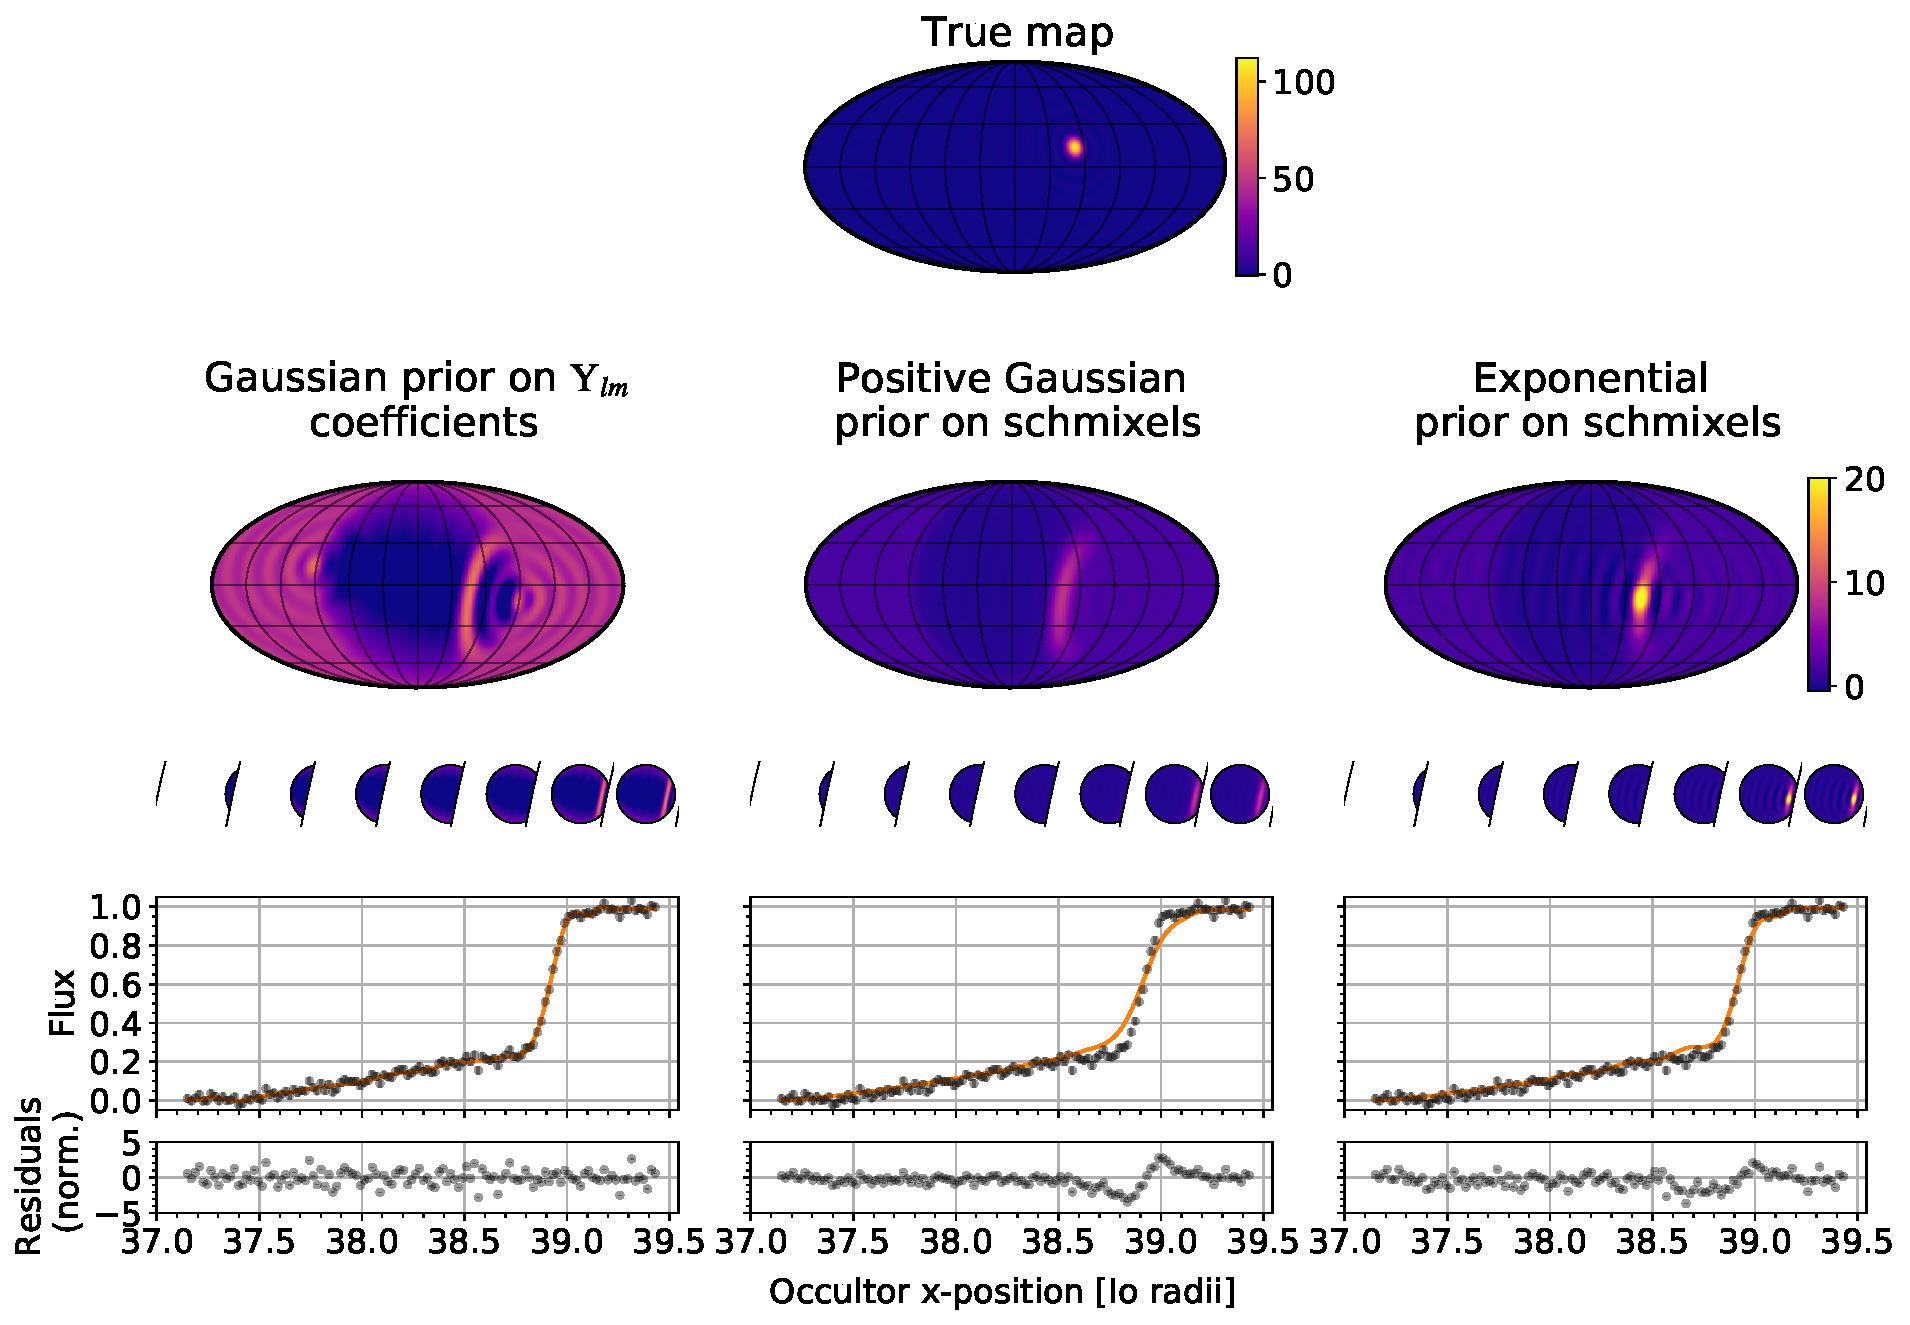
\includegraphics[width=1.\linewidth]{figures/pixels_vs_harmonics.pdf}
    \oscaption{sphixels_vs_harmonics}{%
        Median estimates of $l=20$ maps (second panel from the top) produced by fitting a simulated light curve (bottom) which had been generated from an $l=30$ map consisting of a single bright spot (top). 
        The small circles beneath each inferred map show the progression of the occultation.
        The map on the left corresponds to a model in which we directly fit for spherical harmonic coefficients $\mathbf{y}$ with a Gaussian prior.
        Orange lines show posterior samples in data space and the residuals shown at the bottom are computed with respect to the median of those samples.
        The map in the middle corresponds to a model in which we instead fit for sphixels $\mathbf{p}'$ with a Half Gaussian prior but still use $\mathbf{y}$ to compute the flux.
        The map on the right is the same as the middle one except we use an Exponential prior.
        The scale parameter of the Half Gaussian and the Exponential prior is set to a value which approximates the scale of Gaussian prior on $\mathbf{y}$ to ensure fair comparison between the solutions. 
        The location of the true spot is not recovered correctly because a single light curve does not contain enough information to break the degeneracy in position along the limb of the occultor.
        \label{fig:sphixels_vs_harmonics}
    }
    \end{centering}
\end{figure}

To ensure that the difference in the inferred maps is not in part due to a difference in the scale of the priors, we take 10000 prior samples of the $y$ in the spherical harmonic model, compute the standard deviation and use that as the scale parameter of the Half Gaussian and the Exponential prior.
We implement the model in the probabilistic programming language \textsf{numpyro} (CITE) which is built on top of the \textsf{JAX} library and fit it with Hamiltonian Monte Carlo using the No-U-Turn-Sampler (NUTS) (CITE).
\textsf{JAX} is a \textsf{numpy} like library which supports automatic differentiation, parallelization and GPUs.
We run the chains until for X tuning steps and Y final steps (TODO: HOW MANY?), monitoring divergences and the R-hat  diagnostic to check for convergence.
Because these models have many hundreds if not thousands of parameters, it wouldn't be possible to fit them (at least for nontrivial priors) without automatic differentiation.

The results are shown in Figure~\ref{fig:sphixels_vs_harmonics}.
The top subplot shows the true map with a localized bright spot and the 
inferred maps are shown in the second row from the top together with the progression of the occultation (miniature maps). 
Bottom subplots show the simulated light curves, the predicted flux from the model and the normalized residuals.
The difference between the inferred maps is substantial despite the fact that the predicted flux is similar in all three cases.
The inferred map from the spherical harmonic model (left) has near zero intensity on the observer facing side of Io except for a bright arc tracing the projected limb of Jupiter at the location of the true spot.
The flux on the unobserved side of Io is nearly uniform and significantly higher than the flux on the observer facing side which results in an unrealistic transition between the bright and the dark region at $\pm 90^\circ$ longitude. 
A very clear "ringing" pattern is visible in the with high intensity peaks and low (in some regions negative) intensity troughs.
These features are a consequence of the finite order spherical harmonic expansion of the map and we could in principle get rid of them by fitting a much higher order map but at $l=20$ we are already pushing the limits of what \textsf{starry} can handle.
Besides avoiding unphysical negative intensities, ringing is undesirable because we want to avoid situations in which the model uses the rings to explain the data instead of just placing a spot directly. 
For example, we find that for some fits at low $l$, the model would place a bright spot on the unobserved side of Io in order to produce a ringing artefact on the observed side to explain an increase or decrease in brightness in the light curve. 
This is happening to a lesser extent in the shown map where a small spot is visible at the right edge of the observed hemisphere in order to amplify the visible bright arc through ringing.

The sphixel model with Half Gaussian priors produces a simpler map in which the unobserved hemisphere has much lower intensity but the arc is less sharply defined and more extended and as a result the predicted flux does not rise steeply enough compared to the light curve.
Finally, the Exponential prior on sphixels results in a map with the most spot like feature 
which is somewhat surprising because based on Figure~\ref{fig:sphixels_to_pixels}, we wouldn't expect much difference between the Half Gaussian and the Exponential priors.
It seems that the heavier tail of the Exponential is nevertheless able to induce a sparser solution.
The rightmost map also has the most visible ringing artefacts, an issue which we discuss in the following section.

\subsection{Smoothing out spurious features}
\label{ssec:spurious_features}
To suppress ringing which results in regions of negative intensity surrounding a spot like feature as in Figure~\ref{fig:sphixels_vs_harmonics}, we apply a spatial smoothing filter to the spherical harmonics.
Mathematically, the filtering operation is a convolution between the map and some kernel function $B(\theta,\phi)$.
Assuming both the map and the kernel function are expanded in terms of spherical harmonics, the convolution operation is simply a multiplication between the two sets of spherical harmonic coefficients.
We choose a simple azimuthally symmetric Gaussian kernel function given by
\begin{equation}
    B(\theta)=\frac{1}{\sqrt{2 \pi \sigma_s^{2}}}\exp \left(-\theta^{2} / 2 \sigma_s^{2}\right)
    \quad,
\end{equation}
where $\sigma_s$ sets the characteristic scale of the smoothing.
This function can be expanded in terms of spherical harmonics as
\begin{equation}
    B(\theta)=\sum_{l=0}^{\infty}\left(\frac{2 l+1}{4 \pi}\right) B_{l} \,\mathcal{P}_{l}(\cos \theta)
    \quad,
\end{equation}
where $B_l$ are the spherical harmonic coefficients and $\mathcal{P}_l$ are the associated Legendre polynomials.
They depend only on $l$ because all nonzero $m$ modes vanish due to azimuthal symmetry.
For $\sigma_s\ll 1$ $B_l$ can be approximated as \citep{seon2007,white1995}
\begin{equation}
    B_l\simeq \exp\left[-\frac{1}{2}l(l+1)\sigma_s^2\right]
\end{equation}
The effect of this filter is to exponentially suppress features on scales smaller than $l\sim \sigma_s^{-1}$.

Figure~\ref{fig:smoothing_kernel} shows the effect of (Gaussian) smoothing on a spherical harmonic expansion of a spot with a Gaussian intensity profile.
We place the spot at $0^\circ$ latitude and longitude and set the size of the spot $\Delta\theta$ to $5^\circ$.
All three subplots show the exact profile of the spot (black line) and expansions up to three different orders $l$ (colored lines).
The subplot on the left shows the expansion with no smoothing ($\sigma_s=0$) in which case the symmetric ringing around the center of the spot is clearly visible even at relatively high order ($l=20$).
The middle subplot shows an intermediate level of smoothing where $\sigma_s=0.1$, meaning that all features on scales above $l\approx 10$ are exponentially suppressed.
The negative ringing is a lot less visible albeit at the cost of having a slightly larger spot because suppressing higher order harmonics necessarily means that we lose some ability to represent smaller scale features.
For $\sigma_s=0.2$ (right) there is practically no ringing, but the expansions at $l=10$, $l=15$ and $l=20$ result in the spot of the same size because all coefficients above $l=5$ are significantly suppressed.

\begin{figure}[h!]
    \begin{centering}
    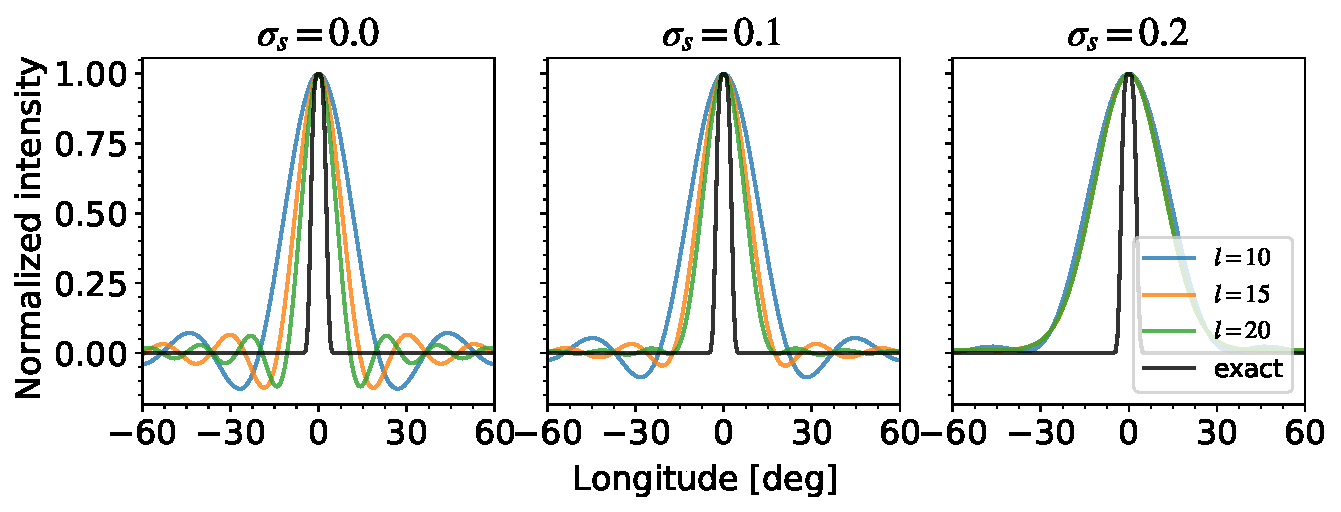
\includegraphics[width=1.\linewidth]{figures/smoothing_kernel.pdf}
    \oscaption{smoothing_kernel}{%
       Normalized intensity of a spherical harmonic expansion of 
        a Gaussian spot placed at $0^\circ$ latitude and longitude.
        The expansion is in the quantity $\cos\Delta\theta$ where $\Delta\theta=5^\circ$.
        The three plots show the spot profile for increasing values of the smoothing parameter 
    $\sigma_s=0$. 
        The colored lines correspond to spot expansions up to a certain order and the black line is the exact expansion.
        The purpose of smoothing is to taper higher order spherical harmonic coefficients in order to suppress ringing artefacts which result in negative intensities.
        High levels of smoothing suppress the ringing completely but as a result they increase the spot size and eliminate differences between expansions above a certain order.
        Intermediate levels of smoothing provide a compromise between the two extremes.
               \label{fig:smoothing_kernel}
    }
    \end{centering}
\end{figure}

Thus, there is a trade-off between smoothing and the ability to resolve smaller scale features
in maps. 
In principle we can always get rid of ringing by fitting sufficiently high order maps.
In practice, computing the analytic integrals computed by \textsf{starry} becomes computationally unstable above $l\approx 25$ so instead of going to very high order we apply some smoothing to mitigate the ringing.
We find that setting $\sigma_s=2/l$ where $l$ is the order of expansion of the map  is a good default setting for $\sigma_s$.

\section{Results for simulated data}
\label{sec:results_sim}
\subsection{Fitting simulated ingress/egress light curves}
\label{ssec:fitting_sim_ingress_egress}
In this section we generalize the simulated example from Section~\ref{ssec:sphixels_vs_harmonics} to include two light curves with 150 data points each.
The first light curve corresponds to an ingress of Io as it is disappearing behind Jupiter and the second light curve corresponds to the egress when Io reappears. 
As before we assume that we know the ephemeris exactly.
The simulated map consists of two spots.
The first spot is located at $13^\circ$ N latitude and $51^\circ$ E longitude and the second spot is at $-15^\circ$ N latitude and $-40^\circ$ E longitude.
Both have the same angular diameter of $15^\circ$.
The amplitude of the bright spot is set to 100\% and the amplitude of the faint spot is to 20\% of the luminosity of the featureless map. 
We generate the light curves from an $l=20$ map and fit a map of the same order and we apply a Gaussian smoothing filter to both the simulated map and the inferred map with the smoothing parameter set to $\sigma_s=2/l=2/20$.
We assume that the phase of Io changes linearly between $10^\circ$ W and $10^\circ$ E the beginning of the ingress and the end of the egress.

We place a sparse prior on the sphixels called the Regularized Horseshoe prior (also known as the "Finnish Horseshoe") \citep{piironen2017}. 
This prior is specifically designed for use in Bayesian sparse linear regression. 
It is an improvement on the Horseshoe prior introduced in \cite{carvalho2010}.
The idea behind the Horseshoe prior is to set the scale for each regression coefficient (sphixel) to a product of a global scale $\tau$ and a local scale $\lambda_m$ where $m$ indexes all the sphixels.
It is defined hierarchically as 
\begin{equation}
\begin{aligned}
    &\tau  \sim \mathrm{Half}-\mathcal{C} \left(0, \tau_{0}\right)\\
    &\lambda_{m}  \sim \mathrm{Half}-\mathcal{C} (0,1) \\
    &p_{m}  \sim \mathcal{N}\left(0, \tau \lambda_{m}\right) 
\end{aligned}
    \quad,
    \label{eq:horseshoe}
\end{equation}
where $p_m$ are the sphixels.
Each local scale parameter is drawn from a unit scale heavy tailed Half Cauchy distribution which allows for very large values of the sphixels.
The global scale parameter is also a free parameter, drawn from a Half Cauchy distribution with the scale equal to $\tau_0$.
The Horseshoe prior is closely related to the spike-and-slab prior which is is a mixture between a delta function prior at zero (\emph{spike}) and some other prior elsewhere (\emph{slab}).

The Regularized Horseshoe prior adds another level to Eq.~\ref{eq:horseshoe} to allow fine tuned control of sparsity and to regularize very large values of coefficients in cases where the data is only weakly constraining.
\cite{piironen2017} show that the Regularized Horseshoe prior can be considered as a continuous counterpart of the spike-and-slab prior with a finite slab width $c$ whereas the Horseshoe prior resembles a spike-and-slab prior with a slab of infinite width.
The Regularized Horseshoe is defined by
\begin{equation}
\begin{aligned}
    &\tau  \sim \mathrm{Half}-\mathcal{C}\left(0, \tau_{0}\right)\\
    &c^{2}  \sim \mathrm{Inv}-\mathcal{G}\left(\frac{\nu}{2}, \frac{\nu}{2} s^{2}\right) \\
    &\overline{\lambda}_{m}  \sim \mathrm{Half}-\mathcal{C}(0,1) \\
    &\lambda_{m} =\frac{c \overline{\lambda}_{m}}{\sqrt{c^{2}+\tau^{2} \overline{\lambda}_{m}^{2}}} \\
    &p_{m}  \sim \mathcal{N}^+\left(0, \tau \lambda_{m}\right) 
\end{aligned}
    \label{eq:reg_horseshoe}
\end{equation}
Integrating out the slab scale $c$ implies a marginal $\mathrm{Student}-\mathit{t}\,(\nu,0,s)$ prior for sphixels far from zero.
When sphixels $p_m$ are close to zero ($\tau^2\overline{\lambda}_m^2\ll c^2$) we have $\lambda_m^2\rightarrow\overline{\lambda}_m^2$ and the prior approaches the original Horseshoe.
When sphixels are far from zero ($\tau^2\overline{\lambda}_m^2\gg c^2$) then $\lambda_m^2\rightarrow c^2/\tau^2$ and the prior approaches $\mathcal{N}(0, c)$.

For setting the scale parameter $\tau_0$ for the prior on the global scale $\tau$, \cite{piironen2017} suggest the following expression
\begin{equation}
    \tau_0=\frac{p_0}{D-p_0}\frac{\sigma}{\sqrt{n}}
    \quad,
    \label{eq:horseshoe_tau0}
\end{equation}
where $p_0$ is our prior guess for the number of significant (sphixels) which are sufficiently far above zero, $D$ is the total number of sphixels, $n$ is the number of data points and $\sigma$ is the standard deviation of the data points (the errobars).
Thus, we only need to specify $p_0$, the degree of freedom parameter $\nu$ and the slab width $c$.

When using the Regularized Horseshoe prior in a small data regime it is often necessary to use the non-centered parametrization to avoid funnels in the posterior which are often present in hierarchical models.
The purpose of this reparametrization is to reduce the dependence between the hyperparameters in the posterior.
To implement the non-centered parametrization we replace priors in Equation~\ref{eq:reg_horseshoe} with zero mean and unit variance priors and rescale them with deterministic transforms as follows
\begin{equation}
\begin{aligned}
    &\overline{\tau} \sim \mathrm{Half}-\mathcal{C}\left(0, 1\right)\\
    &\overline{c^{2}}  \sim \mathrm{Inv}-\mathcal{G}\left(\frac{\nu}{2}, 1\right) \\
    &\overline{\lambda}_{m}  \sim \mathrm{Half}-\mathcal{C}(0,1) \\
    &\overline{p}_{m}  \sim \mathcal{N}^+\left(0, 1\right)\\
    &\tau=\tau_0\overline{\tau}\\
    &c^2=\frac{\nu}{2}s^2\,\overline{c^2}\\
    &\lambda_{m} =\frac{c \overline{\lambda}_{m}}{\sqrt{c^{2}+\tau^{2} \overline{\lambda}_{m}^{2}}} \\
    &p_m = \tau\lambda_m\,\overline{p}_m
\end{aligned}
    \label{eq:reg_horseshoe_noncentered}
\end{equation}
We find that without using the non-centered parametrization the sampling is problematic and there are lots of divergences in the gradients of the parameters, with the non-centered parametrization there are no problems with sampling.

To fully specify the prior, we set $p_0$ to 80\% of the total number of sphixels, $\nu=4$ and $c=10$. 
We fit the model with NUTS with 500 warm-up steps and 1500 final steps. 
The results for a light curve with SNR=50 are shown in Fig.~\ref{fig:ingress_egress_sim_snr_50} and the light curve with SNR=10 are shown in Fig.~\ref{fig:ingress_egress_sim_snr_10}.
For both light curves we recover the locations of the two spots to a high accuracy. 
The inferred bright spot is nearly indistinguishable from the true spot, the fainter spot is somewhat less well constrained but the error in position for both is at most a few degrees.
Rinding artefacts are minimal because we of the smoothing filter.
There are no discernible patterns in the residuals with respect to the median model in data space. 
We found that with priors other than the Horseshoe class priors the model was not able to capture the first step in the light curve which is due to the fainter spot coming in our out of view, it would only recover the brighter spot.
In Fig.~\ref{fig:ingress_egress_sim_snr_10} we show the output of the same model except assuming we have data of worse quality with SNR=10. 
Despite the increased white noise the inferred map does not look substantially different from the one shown in Fig.~\ref{fig:ingress_egress_sim_snr_50}.

\begin{figure}[h!]
    \begin{centering}
    \includegraphics[width=1.\linewidth]{figures/ingress_egress_sim_snr_50.pdf}
    \oscaption{ingress_egress_sim_snr_50}{%
        Median estimate of an $l=20$ map (middle panel) inferred by fitting a pair of simulated ingress/egress occultation light curves of Io assuming SNR=50.
        The simulated map has the same degree as the inferred map and it consists of two hot spots.
The small circles beneath the inferred map show the progression of the occultation. 
        Orange lines show posterior samples in data space and the residuals shown at the bottom are computed with respect to the median of those samples.
With the Regularized Horseshoe prior placed on sphixels, the model is able to recover the locations of both hot spots using only two light curves.
       \label{fig:ingress_egress_sim_snr_50}
    }
    \end{centering}
\end{figure}


\begin{figure}[h!]
    \begin{centering}
        \includegraphics[width=1.\linewidth]{figures/ingress_egress_sim_snr_10.pdf}
    \oscaption{ingress_egress_sim_snr_10}{%
        Same as Fig.~\ref{fig:ingress_egress_sim_snr_50} except for light curves with SNR=10.
       \label{fig:ingress_egress_sim_snr_10}
    }
    \end{centering}
\end{figure}

\subsection{Comparison to a parametric model}
It is instructive to compare the model developed in the previous section to a parametric model in which we assume that the map contains some fixed number of spot and we fit for the positions, amplitudes and the sizes of the spots.
A parametrized spot model might be useful if we want to fit for a small number of spots and we know what the map should look like.
To test how the parametrized spot model compares to the model defined in Section~\ref{ssec:fitting_sim_ingress_egress} we fit it to the light curves shown in Figure~\ref{fig:ingress_egress_sim_snr_50}. 
We then fit a model consisting of 5 parameters: the latitude, longitude, amplitude and size of the spot.
We place uniform priors on the angles and positive Gaussian priors on other parameters. 

We find that if the number of modeled spots matches the number of true spots the model easily converges to the true solution. 
If the number of modeled spots is larger or smaller than the true number the model does not converge due to pathologies in the posterior distribution.
To summarize, although a parametric approach likely would have been sufficient for modeling the light curves shown in this work, it won't work well when the number is unknown or if the features aren't spots and there is no need to restrict ourselves to a parametric model where the sphixel model gives the same results with fewer assumptions about the surface. 
The computational advantages of the parametric spot model relative to the sphixel model are minimal. 
Even though the spot model has only 5 parameters per spot and the sphixel model has thousands of parameters, the runtime for the sphixel model is only longer by a factor of a few. (TODO: add more details to this section).

\section{Results for IRTF data}
\label{sec:results}
\subsection{1998 pair of occultations by Jupiter}
Having demonstrated that our model works well on simulated data, we turn to fitting observations of actual occultation of Io observed with the IRTF telescope.
We selected two pairs of high quality ingress/egress light curves closely spaced in time so that the assumption that the surface map is identical for both the ingress and the egress light curve is approximately correct; although we allow for a difference in the overall amplitude of the maps for the two occultations.
We fit a pair of events from 1998, an ingress occultation observed on the 27th of August and an egress occultation observed on the 29th of November.
For comparison, we also fit a pair of events observed nearly two decades later in 2017.
The predicted fluxes are given by 
\begin{align}
    \mathbf{f}_I&=\mathbf{A}_I'\,\mathbf{p}_I' +b_I\,\mathbf{1}_{N_I}\\
    \mathbf{f}_E&=\mathbf{A}_E'\,\mathbf{p}_E' +b_E\,\mathbf{1}_{N_E}
\end{align}
where $\mathbf{f}_I$ is the predicted flux for the ingress light curve with $N_I$ data points, $\mathbf{f}_E$ is the predicted flux for the egress light curve with $N_E$ data points, and $b_I$ and $b_E$ are constant flux offset parameters.
Since we assume that the map is the same for both light curves up to an overall amplitude difference, we have
\begin{equation}
    \mathbf{p}'_E=a\,\mathbf{p}'_I
    \quad,
\end{equation}
where $a$ is a dimensionless parameter.

The log likelihood is the sum of the log likelihoods for individual light curves (Eq.~\ref{eq:likelihood}), to compute it we also need to specify the data covariance matrix defined in Eq.~\ref{eq:data_covariance_element}.
Each element of the covariance matrix consists of a white noise component (errobars) and a correlated noise component (Gaussian Process).
Since the IRTF light curves are not provided with estimated errobars, we choose to fit for all errobars simultaneously using a hierarhical approach in which we assign a global scale $l$ for all errorbars in a given light curve and we draw each individual errobar from a Half Normal distribution with standard deviation equal to that scale.
That is, we have 
\begin{align}
    \sigma_{i,I}&\sim \mathcal{N}^+(0, l_E),\quad i=1,\dots,N_I\\
    \sigma_{i,E}&\sim \mathcal{N}^+(0,l_I),\quad i=1,\dots, N_E
\end{align}
where $\sigma_{i,I}$ are the errobars for the ingress light curve and $\sigma_{i,E}$ are the errobars for the egress light curve.
Treating errobars as free parameters means that we are introducing hundreds of more parameters (as many as there are data points) which is not an issue as long as these parameters are constrained by the data.

Our noise model as defined above is extremely flexible, it can account for a given feature in the light curve by inflating individual errobars (white noise) or by varying the characteristic timescale $\rho_\mathrm{GP}$ in the Matern 3/2 kernel.
All model parameters and their associated priors are listed in Table~\ref{tab:priors}. 

\renewcommand*{\arraystretch}{1.4}
\begin{table}[t!]
    \begin{center}
        \begin{longtable}{W{l}{4cm} W{l}{4cm} W{l}{6cm}}
            \label{tab:priors}
            \\
            %
            \toprule
            \multicolumn{1}{c}{\textbf{Parameter(s)}}
             &
            \multicolumn{1}{c}{\textbf{Description}}
             &
            \multicolumn{1}{c}{\textbf{Prior}}
            \\
            \midrule
            \endhead
            \bottomrule                                 
            \\
            %
            \caption{%
Parameters and priors for the final model. 
            The subscript $I$ denotes parameters associated with the ingress light curve while the subscript $E$ denotes parameters associated with the egress light curve. $t_{\mathrm{max},I}$ and  $t_{\mathrm{max},E}$ are the durations of the ingress and egress occultations respectively.
            }
            \endfoot
            %
            %
$\tau$ & global sphixel scale &  \begin{minipage}{0.5\textwidth}  \shortstack[l]{$\mathrm{Half}-\mathcal{C}(0,\tau_0)$, $\tau_0$ defined in Eq.~\ref{eq:horseshoe_tau0} \\with $p_0=0.8D$}\end{minipage}
           %
            \\
            %
            $c^2$ & slab scale squared & $\mathrm{Inv}-\mathcal{G}(\frac{\nu}{2},\frac{
                nu}{2}s^2)$, $s=1000$ and $\nu=4$
            %
            \\
            %
    $\overline{\lambda}_m , \quad m=1,\dots,D$  & local sphixel scale & $\mathrm{Half}-\mathcal{C}(0,1)$
            %
            \\
            $p_m, \quad m=1,\dots,D$& sphixels & $\mathcal{N}^+(0, \tau\lambda_m)$, $\lambda_{m} =c \overline{\lambda}_{m}/\sqrt{c^{2}+\tau^{2} \overline{\lambda}_{m}^{2}}$
            %
            \\
            %
                $a$ & \begin{minipage}{0.2\textwidth}\shortstack[l]{relative change in \\map amplitude}\end{minipage}& $\mathcal{N}(1, 0.1)$
             %
            \\
            %
    $b_I$, $b_E$& flux offset &$\mathcal{N}(0, 4)$
            %
            \\
            %
            $l_I$, $l_E$& errorbar global scale&$\mathcal{N}^+(0,0.1)$
            %
            \\
            %
            $\sigma_{i,I}$, $\sigma_{i,E},\quad i=1,\dots,N$& individual errobars&
            $\mathcal{N}^+(0,l_I),\quad \mathcal{N}^+(0,l_E)$
            %
            \\
            %
            $\sigma_{\mathrm{GP}, I}$, $\sigma_{\mathrm{GP}, I}$ & GP standard deviation&$\mathcal{N}^+(0,0.1),\quad \mathcal{N}^+(0,0.1)$
             %
            \\
            %
            $\rho_{\mathrm{GP},I}$, $\rho_{\mathrm{GP},E}$ & GP timescale  & $\mathcal{N}^+(0, t_{max, I}),\quad  \mathcal{N}^+(0, t_{max, E})$
        \\
            %
        \end{longtable}
    \end{center}
\end{table}

To fit the model we sample the posterior using the NUTS sampler for 500 warm-up steps and 3000 final steps.
We monitor divergences and the R-hat statistic to ensure convergence.
The inferred map for the 1998 pair of events is shown in Figure~\ref{fig:irtf_ingress_egress_1998} and the median, 16th and 84th percentile estimates from the samples are shown in Table~\ref{tab:irtf_1998}. 
The inferred map has two distinct hot spots, a bright hotspot in the Eastern hemisphere and a faint hotspot in the Western hemisphere.
The orange lines in the second panels from the bottom are posterior samples for the physical (map) model in data space. 
The bottom panel shows the residuals with respect to the (median) physical model prediction and the posterior predictions from the Gaussian Process (purple).
We plot the model in this way so that we are able to distinguish between the features due to the physical model and those from the noise model.
Each data point is shown with the median prediction of its errorbar.

\begin{figure}[ht!]
    \begin{centering}
    \includegraphics[width=1.\linewidth]{figures/irtf_ingress_egress_1998.pdf}
    \oscaption{irtf_ingress_egress_1998}{%
    Median estimates of two $l=20$ maps (top panel) inferred by fitting a pair of observations of occultations of Io by Jupiter from 1998.  
        The map and light curve on the left correspond to the ingress event and the ones on the right are the egress event. 
        The two maps are (by construction) the same except for a difference in the overall amplitude. 
The small circles beneath the inferred map show the progression of the occultation. 
        Orange lines show posterior samples from the physical model.
        The residuals (bottom) are computed with respect the median prediction from the physical model and the Gaussian Process posterior predictions are shown on the same plot in purple.
        The inferred map shows two hotspots, the bright hot spot is emission due to Loki and the faint hot spot is Kanehekili (TODO: check).
     \label{fig:irtf_ingress_egress_1998}
    }
    \end{centering}
\end{figure}

Despite the fact that our noise model is very flexible, it does not seem to overfit the data. 
The physical model accounts for the prominent steps in the light curves while the noise model takes care  of the residual variability. 
Most of the wiggles in the residuals are either due to surface emission features which were not accounted for by the model or due to atmospheric variability.
The most notable feature in the residuals is visible at around 3.3 minutes in the ingress light curve and 3.6 minutes in the egress light curve when the bright hot spot comes in and out of view. 
This feature is visible because our model is limited in resolution so the inferred spot size is not small enough to explain the rapid change in flux seen in the data.
The Gaussian Process accounts for the  variation due to atmospheric variability, the emission due to surface features which are too faint to be well constrained by the physical model and the limitation of the physical model to capture the true size of the spot. 

There is a trade-off between the explanatory power of the noise model and the physical model. 
In general, we expect that a given feature in the light curve will be accounted for by the physical model if the physical model provides a better explanation for the data relative to the noise model.
This seems to be true for the most obvious features in Figure~\ref{fig:irtf_ingress_egress_1998} except (to an extent) for the first step in the ingress light curve at around 0.6 minutes which is only partially accounted for by the physical model because the model predictions are a bit too smooth compared to the data. 
Based on the ingress light curve alone, we would expect that the faint spot should be slightly brighter than the model predicted.
Since the model had no trouble accounting for a similar a step for simulated data shown in Figure~\ref{fig:ingress_egress_sim_snr_50} the reason why it didn't do so in this case is probably because doing so would result in a poorer fit for the egress light curve.
The two occultations were observed months apart so we expect our assumption that the map has not changed except for an overall amplitude to be wrong in detail.  

The posterior distribution for the errobars is shown in Figure~\ref{fig:irtf_ingress_egress_errorbars}.
Both the global scale for the errobars and the individual errobars are well constrained by the data. 
Looking at the plot one can see that outlier points are naturally accounted for in the model because those points end up having higher variance.

\begin{figure}[ht!]
    \begin{centering}
    \includegraphics[width=\linewidth]{figures/irtf_ingress_egress_1998_errobars.pdf}
    \oscaption{irtf_ingress_egress_errobars}{%
       \label{fig:irtf_ingress_egress_errorbars}
    }
    \end{centering}
\end{figure}

\renewcommand*{\arraystretch}{1.4}
\begin{table}[t!]
    \begin{center}
        \begin{longtable}{W{l}{2cm} W{l}{3cm} W{l}{3cm}}
            \label{tab:irtf_1998}
            \\
            %
            \toprule
            \multicolumn{1}{c}{\textbf{Parameter}}
             &
            \multicolumn{1}{c}{\textbf{Value}}
             &
            \multicolumn{1}{c}{\textbf{Unit}}
            \\
            \midrule
            \endhead
            \bottomrule                                 
            \\
            \caption{%
                Inferred parameters for the pair of occultations observed in 1998 using the IRTF telescope.
                }
            \endfoot
            $\tau$ &   $0.870_{-0.221}^{+0.246}$ &  intensity
            \\
             $c$ & $4304.302_{-1162.250}^{+2123.962}$ & intensity 
            \\
                $a$ &  $1.154_{-0.013}^{+0.014}$ & dimensionless
            \\
            $b_I$ & $0.014_{-0.013}^{+0.077}$ & GW/um/sr
            \\
            $b_E$& $0.362_{-0.335}^{+0.438}$ & GW/um/sr
            \\
            $l_I$ & $0.253_{-0.030}^{+0.036}$ & GW/um/sr
            \\
            $l_E$& $0.461_{-0.042}^{+0.042}$ & GW/um/sr
            \\
            $\sigma_{\mathrm{GP}, I}$ & $0.633_{-0.042}^{+0.047}$ & GW/um/sr 
            \\
            $\sigma_{\mathrm{GP}, E}$ & $0.453_{-0.052}^{+0.054}$ & GW/um/sr
            \\
            $\rho_{\mathrm{GP},I}$ & $0.078_{-0.010}^{+0.011}$ & minutes
            \\
            $\rho_{\mathrm{GP},E}$ & $0.099_{-0.021}^{+0.027}$ & minutes
            \\
        \end{longtable}
    \end{center}
\end{table}

To obtain the inferred location of both hot spots, we compute the centroid of pixels in the 90th percentile of intensity (meaning the brightest pixels) in a specific region (in latitude and longitude) around the hot spot. 
We repeat this for each posterior map to obtain uncertainty on the position. 
In addition to the locations of the spots, we also compute the total power emitted within a 15 degree range in latitude and longitude around the (inferred) center of the spots.
Both of these quantities are listed in Table~\ref{tab:irtf_1998_derived}. 
The location of the bright hotspot is $16.414_{-0.011}^{+0.027}\quad^\circ$ N latitude and $53.107_{-0.033}^{+0.041}\quad^\circ$ E longitude which corresponds to the location of Loki Patera.
The faint hot spot is at $-15.756_{-11.382}^{+3.812}\quad ^\circ$ N latitude and $321.568_{-4.208}^{2.803}\quad^\circ$ E longitude which is most likely Kanehekili (TODO: check if this is true).
Figure~\ref{fig:irtf_ingress_egress_spots} shows  a contour map of both hot spots overlaid on top of the U.S. Geological Survey's map of the surface of Io \cite{williams2011} which was constructed from Galileo observations.
Also shown is the inferred error in position (white lines).
The error on the inferred position of Loki is only a fraction of a degree and thus much smaller than the minimum resolution of the map features which is set by the degree of the map.
TODO: Mention the uncertainty due to Jupiter's radius.

\renewcommand*{\arraystretch}{1.4}
\begin{table}[t!]
    \begin{center}
        \begin{longtable}{W{l}{4cm} W{l}{3cm} W{l}{3cm}}
            \label{tab:irtf_1998_derived}
            \\
            %
            \toprule
            \multicolumn{1}{c}{\textbf{Parameter}}
             &
            \multicolumn{1}{c}{\textbf{Value}}
             &
            \multicolumn{1}{c}{\textbf{Unit}}
            \\
            \midrule
            \endhead
            \bottomrule                                 
            \\
            \caption{%
                Derived parameters of the two hot spots visible in Figure~\ref{fig:irtf_ingress_egress_1998}.
                The latitude and longitude of the spots are derived by computing the centroid of points around the spots which are in the 90th percentile of intensity.
            The power is defined as the total emission from within a 15 degree circle around the (inferred) location of the spot.
        }
            \endfoot
            Spot 1 latitude  & $16.414_{-0.011}^{+0.027}$& degrees 
            \\
             Spot 1 (East) longitude & $53.107_{-0.033}^{+0.041}$& degrees 
            \\
                Spot 1 power  ingress & $52.755_{-0.316}^{+1.090}$ & GW/um 
            \\
                Spot 1 power  egress & $61.055_{-1.000}^{+1.081}$ & GW/um 
                \\
            Spot 2 latitude  & $-15.756_{-11.382}^{+3.812}$& degrees 
            \\
             Spot 2 (East) longitude & $-38.432_{-4.208}^{+2.803}$ & degrees 
            \\
                Spot 2 power  ingress & $5.192_{-15.95}^{+0.484}$ & GW/um 
                \\
                Spot 2 power  egress & $6.026{-1.993}^{+0.534}$ & GW/um 
            \\
        \end{longtable}
    \end{center}
\end{table}

\begin{figure}[ht!]
    \begin{centering}
    \includegraphics[width=\linewidth]{figures/irtf_ingress_egress_1998_spots.pdf}
    \oscaption{irtf_ingress_egress_1998_spots}{%
        Contour plot of the hot spots shown in Figure~\ref{fig:irtf_ingress_egress_1998} overlaid on top of the U.S. Geological Survey's map of the surface of Io which has been constructed from observations by the Galileo spacecraft.
        \label{fig:irtf_ingress_egress_spots}
    }
    \end{centering}
\end{figure}

To see how the results change if we don't include a Gaussian Process in the noise model we fit the same pair of occultations from 1998 using the same priors.
The results are shown in Figure~\ref{fig:irtf_ingress_egress_1998_no_GP}.
The model tries to account for the systematic variations in the data by inflating the individual errorbars.
Compared to the map shown in Figure~\ref{fig:irtf_ingress_egress_1998} the map has two spurious extra spots. 
We find that in general including a GP results in a simpler map with fewer features because the GP prevents the physical model from overfitting the data.

\begin{figure}[ht!]
    \begin{centering}
    \includegraphics[width=1.\linewidth]{figures/irtf_ingress_egress_1998_no_GP.pdf}
    \oscaption{irtf_ingress_egress_1998_no_GP}{%
        Same as Figure~\ref{fig:irtf_ingress_egress_1998} except this figure shows the output of a model which does not include a Gaussian Process to account for correlated structure in the data.
    As a result, the model tries to account for the correlations by inflating individual errorbars. 
    There are two additional hot spots which are almost certainly spurious.
     \label{fig:irtf_ingress_egress_1998_no_GP}
    }
    \end{centering}
\end{figure}

\subsection{2017 pair of occultations by Jupiter}
To see what happens if we use the same model as the one used to generate the map shown in Figure~\ref{fig:irtf_ingress_egress_1998} to fit a pair of observations from 2017, an ingress occultation observed on the 31st of March and an egress occultation observed on the 11th of May.
The results are shown in Figure~\ref{fig:irtf_ingress_egress_2017} and the inferred parameters are listed in Table~\ref{tab:irtf_2017}.
The inferred map is very similar to the one shown in Figure~\ref{fig:irtf_ingress_egress_1998} because we again see two hot spots although the fainter one is located a higher latitude.
A contour plots of the two spots overlaid on top of a surface map of Io from Galileo observations is shown in Figure~\ref{fig:irtf_ingress_egress_spots_2017} and the derived spot parameters are listed in Table~\ref{tab:irtf_2017_derived}.

\begin{figure}[ht!]
    \begin{centering}
    \includegraphics[width=1.\linewidth]{figures/irtf_ingress_egress_2017.pdf}
    \oscaption{irtf_ingress_egress_2017}{%
    Median estimates of two $l=20$ maps (top panel) inferred by fitting a pair of observations of occultations of Io by Jupiter from 2017.  
        The map and light curve on the left correspond to the ingress event and the ones on the right are the egress event. 
        The two maps are (by construction) the same except for a difference in the overall amplitude. 
The small circles beneath the inferred map show the progression of the occultation. 
        Orange lines show posterior samples from the physical model.
        The residuals (bottom) are computed with respect the median prediction from the physical model and the Gaussian Process posterior predictions are shown on the same plot in purple.
        The inferred map shows two hotspots, the bright hot spot is emission due to Loki and the faint hot spot is Kanehekili (TODO: check).
                \label{fig:irtf_ingress_egress_2017}
    }
    \end{centering}
\end{figure}


\renewcommand*{\arraystretch}{1.4}
\begin{table}[t!]
    \begin{center}
        \begin{longtable}{W{l}{2cm} W{l}{3cm} W{l}{3cm}}
            \label{tab:irtf_2017}
            \\
            %
            \toprule
            \multicolumn{1}{c}{\textbf{Parameter}}
             &
            \multicolumn{1}{c}{\textbf{Value}}
             &
            \multicolumn{1}{c}{\textbf{Unit}}
            \\
            \midrule
            \endhead
            \bottomrule                                 
            \\
            \caption{%
                Inferred parameters for the pair of occultations observed in 1998 using the IRTF telescope.
                }
            \endfoot
            $\tau$ &   $0.973_{-0.247}^{+0.255}$ &  intensity
            \\
             $c$ & $5866.860_{-1580.812}^{+2527.995}$ & intensity 
            \\
                $a$ &  $1.434_{-0.010}^{+0.011}$ & dimensionless
            \\
            $b_I$ & $0.025_{-0.024}^{+0.140}$ & GW/um/sr
            \\
            $b_E$& $1.026_{-0.263}^{+0.238}$ & GW/um/sr
            \\
            $l_I$ & $0.971_{-0.056}^{+0.056}$ & GW/um/sr
            \\
            $l_E$& $0.520_{-0.093}^{+0.079}$ & GW/um/sr
            \\
            $\sigma_{\mathrm{GP}, I}$ & $0.126_{-0.055}^{+0.129}$ & GW/um/sr 
            \\
            $\sigma_{\mathrm{GP}, E}$ & $0.601_{-0.093}^{+0.083}$ & GW/um/sr
            \\
            $\rho_{\mathrm{GP},I}$ & $2.160_{-2.030}^{+3.333}$ & minutes
            \\
            $\rho_{\mathrm{GP},E}$ & $0.020_{-0.013}^{+0.011}$ & minutes
            \\
        \end{longtable}
    \end{center}
\end{table}


\begin{figure}[ht!]
    \begin{centering}
    \includegraphics[width=\linewidth]{figures/irtf_ingress_egress_2017_spots.pdf}
    \oscaption{irtf_ingress_egress_2017_spots}{%
        Contour plot of the hot spots shown in Figure~\ref{fig:irtf_ingress_egress_2017} overlaid on top of the U.S. Geological Survey's map of the surface of Io which has been constructed from observations by the Galileo spacecraft.
        \label{fig:irtf_ingress_egress_spots_2017}
    }
    \end{centering}
\end{figure}


\renewcommand*{\arraystretch}{1.4}
\begin{table}[t!]
    \begin{center}
        \begin{longtable}{W{l}{4cm} W{l}{3cm} W{l}{3cm}}
            \label{tab:irtf_2017_derived}
            \\
            %
            \toprule
            \multicolumn{1}{c}{\textbf{Parameter}}
             &
            \multicolumn{1}{c}{\textbf{Value}}
             &
            \multicolumn{1}{c}{\textbf{Unit}}
            \\
            \midrule
            \endhead
            \bottomrule                                 
            \\
            \caption{%
                Derived parameters of the two hot spots visible in Figure~\ref{fig:irtf_ingress_egress_2017}.
                The latitude and longitude of the spots are derived by computing the centroid of points around the spots which are in the 90th percentile of intensity.
            The power is defined as the total emission from within a 15 degree circle around the (inferred) location of the spot.
        }
            \endfoot
            Spot 1 latitude  & $12.319_{-0.388}^{+0.391}$& degrees 
            \\
             Spot 1 (East) longitude & $52.743_{-0.095}^{+0.046}$& degrees 
            \\
                Spot 1 power  ingress & $70.719_{-0.275}^{+1.396}$ & GW/um 
            \\
                Spot 1 power  egress & $102.026_{-1.459}^{+1.737}$ & GW/um 
                \\
            Spot 2 latitude  & $-8.076_{-0.084}^{+0.715}$& degrees 
            \\
             Spot 2 (East) longitude & $-42.096_{-0.161}^{+0.417}$ & degrees 
            \\
                Spot 2 power  ingress & $4.513_{-0.742}^{+0.689}$ & GW/um 
                \\
                Spot 2 power  egress & $6.483{-1.059}^{+0.944}$ & GW/um 
            \\
        \end{longtable}
    \end{center}
\end{table}



\section{Conclusions}
\label{sec:conclusions}
\clearpage

% Bibliography
\bibliography{bib}

\end{document}
